\chapter{Modular Run-Time}
\section{Objectives}

The main objective of this work is to create a prototype of a run-time that will have no dependencies on any external libraries, not even the POSIX ones, allowing the developer to set up his own run-time from different modules.

Also, no constructs that require any OS support (dynamic loader, standard OS libraries, etc.) will be used. This means, that constructs such as \verb=static\ __thread= (which creates a new copy of the variable declared for each thread created) or \newline{} \verb=__attribute__((constructor))= (which marks the function to be called by the dynamic loader right after the binary has been loaded) can be used either.

This will, however, requires the user to call some run-time initializing functions manually at the beginning of the program's execution, as they won't get called by the dynamic loader. On systems that do support the constructor functions, this can be easily avoided by compiling the run-time with an additional file which will declare and implement a constructor, as can be seen in the \verb=posix.c= file, which is included with the run-time as an extra, which demonstrates how to add support for your operating system.

In a real-world scenario, of course, we cannot require that each user supplies all these functions first thing in the \verb=main= function. For example, on \verb=*nix=\footnote{Most Unix systems, cannot be guaranteed that this will work on all of the systems.} systems, this can be easily solved by compiling the library with a single \verb=.c= file which has a function populating the setup structure with system-specific functions. This function can then either be called by the dynamic loader (which requires support from the dynamic loader), or can have a GCC-specific \verb=__attribute__((constructor))= if the system supports it. If neither is an option, then the user really needs to call this system-specific function to populate the run-time setup and then initialize the run-time, if the system-specific function hasn't done so. An example of this can be found in the \verb=posix.c= file which is bundled with the run-time as an example.


\subsection{Example 1: Lock-less run-time}
In a single-threaded application (or applications, where you know that Objective-C code will be used only in one thread), there is no need for any locking whatsoever. All of the existing implementations require some locking, even though they are trying to use lock-free structures, such as sparse arrays that do not support deleting.

But even so, any \verb=@synchronized(obj)= code is translated to actually lock a mutex associated with \verb=obj=, be it either a mutex from a lock pool in the traditional run-times, or a mutex that is associated just with \verb=obj= in the \'Etoil\'e run-time. This can speed up both loading of the application and code execution.

\subsection{Example 2: Kernel usage}

To get the existing run-times working in a kernel of an operating system might be tricky, depending on how much is the kernel POSIX-compatible. But even so, the \verb=malloc= functions and others usually are just wrappers around kernel allocators, which slows down allocation of all structures within the run-time.

Using the modular run-time it will be possible to change the allocator with a simple function-pointer assignment.


\subsection{Example 3: Benchmarking}

The modularity that will be introduced by this work will allow anyone to explore changes in the speed of the run-time simply by changing internal data structures used to hold the class list, selector list and caching. This may help the future development of the run-time.


\section{Run-time Setup}

As has been mentioned before, the run-time has been designed to be as flexible as possible. This means that all possible dependencies had to be removed, as well as all assumptions about the underlying OS, or whether the run-time is running in user space, or kernel space.

The run-time, however, needs a way to allocate memory, locks, and so on, which are system-specific tasks. The intention behind this run-time is to completely separate these dependencies, so that porting the run-time on another platform is as easy as providing one single file containing all necessary resources.

There are basically two ways of doing so:

\subsection{Inline Functions}
The first one is very similar to what the other run-time implementations have done - create a header file that contains multiple static inline functions that implement all the OS-specific calls required by the run-time.

This approach to the platform-independence problem has one advantage and one disadvantage. The obvious disadvantage is that you can perform compile-time changes only. Once the run-time has been compiled, there is no way to change, for example, the allocator without performing some wild hackery exchanging the \verb=malloc= function pointer using the dynamic loader API.

The advantage, on the other hand, is definitely speed. There is no extra cost associated with calling these system APIs as the functions get inlined.

\subsection{Function Pointers}

Other approach is to create a setup structure that consists of function pointers, which are then called by the run-time. This has the opposite advantages and disadvantages as inlining functions.

The advantage is that the run-time can be compiled without knowing the functions at all and then every program can decide which allocators to use, etc. Or if there is enough support from the dynamic loader, the dynamic loader can decide which functions to use to populate the run-time setup based on some binary flags.

The dynamic loader could then define a specific function name, \newline{}\verb=objc_runtime_user_preflight()= for example, and if the loaded program had such a function implemented, it would get called before initializing the run-time as that's the point the setup structure needs to be sealed to prevent any further changes in the function pointers as some structures might already be allocated and initialized. If the function pointers were to be changed, it would probably lead to a crash.

The disadvantage here, on the other hand, is speed. While the function itself has to be called anyway, it is possible that the function types used in the run-time do not match function types in your system. You then need to create a proxy function that converts parameters.

For example, the read/write lock functions are made to be compatible with the POSIX \verb=pthread_rwlock_*= functions (as can be seen in \verb=extras/posix.c=), which return an \verb=int= containing a possible error value, or zero if the call was successful. In the same manner, the run-time assumes that if the function pointer returns zero, the call was successful. If the OS you are porting the run-time to doesn't return anything, or returns a different value than zero for success, you need to create a proxy function that calls the system function and then returns some value accordingly. This, however, costs an extra function call.

\subsection{Implementation}

The run-time prototype that is part of this work is designed to support both solutions. Hence if you decide that you want to choose speed over flexibility and dynamic nature of the run-time, you can do so.

The key to this is the \verb=os.h= header file. An \verb#if-#else= divides the file into two parts, one for the inlining support, second one for the function pointers support.

When compiling the run-time, you can switch between these two simply by redefining the \verb=OBJC_USES_INLINE_FUNCTIONS= value - \verb=0= for function pointers, \verb=1= for inline functions.

\paragraph{Inlining}

The first part of the \verb=os.h= header file is the part that should be used for static inline functions. A rough sketch of how this should be used has been included:

\begin{verbatim}
#if TARGET_MY_OS
  #include "os-my-os.h"
#else
  #error "This OS isn't supported at the moment."
#endif
\end{verbatim}

You should hence create your own header file for that particular OS and include it in the run-time source files. The obvious disadvantage here is that you need to supply all necessary functions at the compile time.

For a list of function names required to implement, see the function pointers part, which uses \verb=#define=s to substitute the function names with fetching function pointers from a private structure.

\paragraph{Function Pointers}

If you decide to use function pointers, you don't need to modify the run-time source code at all. The second part of the \verb=os.h= header file is filled with \verb=#define=s that fetch the corresponding function pointer. For example:

\begin{verbatim}
#if OBJC_USES_INLINE_FUNCTIONS

#include <stdlib.h>

// Static-inline allocator, simply passing the call
// to malloc
static inline void *objc_alloc(unsigned int size){
  return malloc(size);
}

#else

#include "runtime-private.h"

#define objc_alloc objc_setup.memory.allocator

#endif

\end{verbatim}

The run-time defines a \verb=objc_setup= global variable in \verb=runtime.c= and exports it in \verb=runtime-private.h=:
 
\begin{verbatim}
objc_runtime_setup_struct objc_setup;
\end{verbatim}

- while the user has no direct access to this structure as it is exported in a private header, the run-time itself can access it directly for the sake of the speed to eliminate unnecessary function calls that would serve just as proxy calls. The user doesn't have a direct access to the structure only as a security precaution so that the structure cannot be modified from the outside during the program execution, but the user is free to get the setup structure using the \verb=objc_runtime_get_setup= function, which copies over the whole setup structure. The user can then cache this structure for performance.

You can view the structure below:

\begin{verbatim}
  // TODO: paste the final structure when available
typedef struct {
  objc_abort abort;
  objc_allocator allocator;
  struct {
    objc_class_holder_creator creator;
    objc_class_holder_destroyer destroyer;
    objc_class_holder_lookup lookup;
  } class_holder;
} objc_runtime_setup_struct;
\end{verbatim}

This allows the modularity of the run-time. One can, at the beginning of his program, modify all of those pointers using setter functions declared in \verb=function-types.h=. After the runtime has been initialized, however, the whole structure is sealed from changes using those setter functions to prevent any data corruption (as some data structures may be already initialized, changing these functions would most likely lead to bad memory access crashing the program). Using any of the setter functions after the run-time has been initialized will lead abort the program.

A description of each section of the setup structure can be found below:

\paragraph{execution}

This part of the structure contains function pointers to functions dealing with the execution of the program itself - it is commonly said that there is no software without bugs - hence it is sometimes necessary to abort the program execution if the program gets into an inconsistent point, or a point where illegal arguments are passed to the environment (for example, setting the run-time setup structure to NULL), hence it contains functions like \verb=objc_abort=, etc.

\paragraph{Allocator, Deallocator, Reallocator and Zero-allocator}

As the run-time needs new memory for dynamic object creation, an allocator is needed. All existing run-times use \verb=malloc=, which, however, ties them to Unix-based operating systems.

The Modular Run-Time lets you specify your own allocator, which can be, for example, just a wrapper around \verb=malloc= adding some debug logging, or a completely different allocator, e.g.\ a kernel allocator as has been mentioned before. It can also be just the \verb=malloc= function itself, as the function type takes just one argument - the size of the memory required and returns a \verb=void*= pointer.

Sometimes, the memory acquired should be filled with zeros - just as the \verb=calloc= function would do, however, it is called \verb=zero_allocator= in this run-time. The \verb=calloc= function can be assigned, however.

For dynamically growing structures, reallocation may be needed - hence the inclusion of the reallocating function. It is pointer-compatible with the \verb=realloc= function.

When the run-time is done with memory it has allocated, it will deallocate it using the deallocate function, which has the same signature as the POSIX \verb=free= function.

\paragraph{Arrays}

A lot of the code of the traditional run-times is riddled with code that is takes care of consistency of dynamically growing arrays (or rather arrays of arrays) - there's a lot of duplicate code for functions related to lists of methods, protocols, etc.\ on each class.

This run-time declares a \verb=objc_array= type, which is just a retyped \verb=void*=, but can be implemented in any possible way. The run-time includes a working implementation of such an array and installs these function pointers at initialization, unless other pointers are provided.

The default implementation is a structure that contains two \verb=unsigned int=s - one that remembers the allocated capacity of the array, the second one pointing to an index in the actual allocated array holding the items. If the structure is initialized as lock-able, then a mutex is allocated as well.


\paragraph{Class Holder}

The run-time needs to keep track of all classes that are registered with it. To do so, it needs to keep a list in some data structure. As the run-time is designed to be flexible, it doesn't matter what data structure at all.

There is a defined data type \verb=objc_class_holder= which, however, is again only a retyped \verb=void*=. Using the run-times function pointers \verb=class_holder.creator=, \verb=class_holder.destroyer=, \verb=class_holder.lookup= and TODO, the run-time creates the data structure required, has means to destroy it, lookup a class according to its name and TODO.

The run-time provides a default implementation of this structure, a simple hash table which resembles slightly \verb=NXMapTable= from Apple's run-time, but removes all dependencies and is made slightly less complicated.

\section{Class}

At the core of the run-time lies a structure representing a class. Like the \'Etoil\'e run-time, this run-time doesn't provide a class pair - a class and its meta-class, but only a single class object that contains class methods as well. While it abandons the Smalltalk similarities, it provides greater flexibility, allowing the Objective-C class structure to be used for other languages as well.

\subsection{Structure of a Class}

The class structure begins in the traditional fashion with a pointer to its superclass - the \verb=isa= pointer. This pointer is followed by the class name, class methods and instance methods. Both class methods and instance methods use the \verb=objc_array= structure, which is a list of lists of \verb=Method=s, just like in the other run-times 

// TODO: cache, ivars

\section{Extensibility of Classes}

While the other run-times allow the user to specify extra space when allocating both a class and an object, it is very limiting as if you want to add this extra space, you need to replace the \verb=+alloc= method of \verb=NSObject=, but even so, it will not affect all classes in the run-time as not all objects are subclasses of \verb=NSObject= (e.g.\ \verb=NSProxy=).

This is why the modular run-time has introduced class extensions which allow developers to extend the run-time capabilities dynamically. Class extensions can be compared to the run-time delegates. The class extensions must get registered using the \verb=objc_class_add_extension()= function before the run-time gets initialized.

This function has a single argument: a pointer to a \verb=objc_class_extension= structure:

\begin{verbatim}
  typedef struct _objc_class_extension {
    struct _objc_class_extension *next_extension;

    void(*class_initializer)(Class, void*);
    void(*object_initializer)(id, void*);
    void(*object_deallocator)(id, void*);
	
    unsigned int extra_class_space;
    unsigned int extra_object_space;
	
    unsigned int object_offset;
} objc_class_extension;
\end{verbatim}

The first field, \verb=next_extension= is a pointer to the next extension as the run-time keeps class extensions in a linked list. The run-time populates this field automatically.

This field is followed by three function pointers:

\begin{itemize}
  \item \verb=class_initialize= - this function gets called each time a class is registered with the run-time using \verb=objc_finish_class()=. This is the place where the extra space, to which a pointer is passed as the second argument, should get populated and initialized.
  
  \item \verb=object_initializer= - any time an object is allocated, this function gets called in order to initialize the extra space in the object (again, the second argument is a pointer to the extra space within the structure).
  
  \item \verb=object_deallocator= - before the object gets deallocated, each class   extension is provided an option to deallocated any dynamically allocated structures.
\end{itemize}

These pointers are followed by three unsigned integers. The first two declare how much space is requested by this class extension for the class and object structures.

The last field is populated by the run-time, when it is being initialized and tells the extension what is the offset in the extra space for this particular extension. When multiple extensions are installed, the extra space is divided among all the extensions. The following image illustrates this scenario: \newline{}

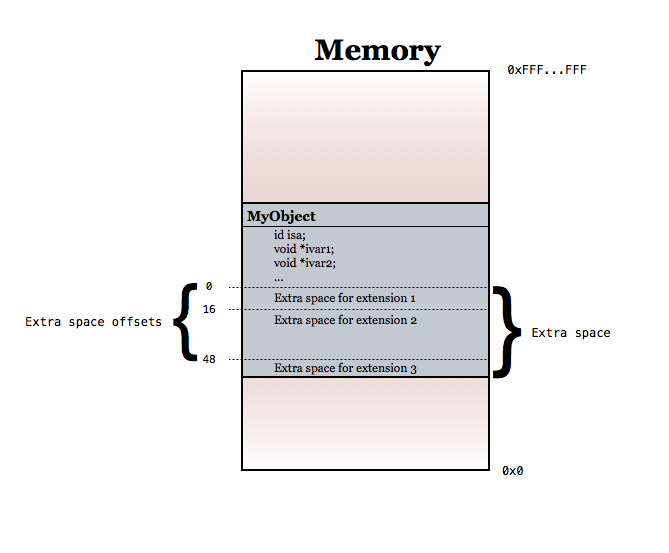
\includegraphics[width=120mm]{img/class_extensions.png}

While it allows to extend the classes with new functionality, for example properties, or ARC (the \verb=object_deallocator= can do all the automatic deallocations), it poses an issue at the compile time - how much extra space should be left? The compiler needs to know the size of the class structure to generate.

One option is to re-allocate all classes with the extra space and copy over all pointers of the class internal structures (it is enough to copy over pointers as the memory will be kept alive). Assuming 1000 classes in a larger application, each class having 64 bytes + those extra bytes, this gives 64 kB of extra memory per application. While this isn't that much nowadays, it would slow down the application launch.

Other option is to dynamically allocate the extra space for each class, so the class structure stays of the same size, with the extra space being outside of the structure itself. This allows to add class functionality without the compiler support and without recompiling any previous classes (note that this applies only to classes - when allocating objects, we can compute the object size as it is not allowed to add class extensions after the run-time has been initialized).

There is an example bundled with the run-time: associated objects (see \verb=extras/associated_objects.c=).

\subsection{Associated Objects}

Since OS X 10.6, Apple's run-time allows to simulate addition of variables to an object using associated objects\footnote{http://developer.apple.com/library/ios/#documentation/cocoa/conceptual/objectivec/chapters/ocAssociativeReferences.html}. It allows you to specify an object for a key (which is \verb=void*=). Simply said, each object has a hash map, where it stores objects.

With the class and object extensions, it is fairly easy to achieve. The class itself doesn't need to be modified at all, hence the \verb=class_initializer= may be \verb=NULL= or a no-op function and \verb=extra_class_space= should be set to 0.

The \verb=extra_object_space= can be set to \verb=sizeof(void*)= in case you want to allocate the hash-table structure dynamically, or something else, if you want to inline the structure.

If you want to lazily create the hash-table, the \verb=object_initializer= can be \verb=NULL= or a no-op function as well and the \verb=object_deallocator= should simply deallocate the hash-table structure if it were ever created.

Then you can create some getter and setter functions for associated objects. To access the hash-table from an \verb=id object=, you can use code similar to the following:

\begin{verbatim}
  // Static declaration of the extension
  static objc_class_extension 
      associated_objects_extension = { ... }

  // At the beginning, the extension gets added to the run-time
  objc_class_add_extension(&associated_objects_extension);

  // Hash table is retrieved
  void *hashtable = ((void*)id) + id->isa->instance_size 
        + associated_objects_extension.object_extra_space_offset;
        
  // Do something with the hashtable
\end{verbatim}


\subsection{Performance}
Just like anything, even adding class extension effects the performance somehow. If no extensions are installed in the run-time, the objects are created directly. If extensions get installed, the extension list needs to be iterated and for each extension, one extra function call is performed. This iteration itself doesn't change the asymptotic complexity as the number of class extensions is constant number, usually a very small one. The only thing that can effect the performance is the object initializer function itself.

To speed things up even more for extensions that lazy-initialize their structures (as described in the Associated Objects example), the run-time allows for any of the function pointers to be \verb=NULL= (this includes the \verb=object_deallocator= if your extension doesn't have to allocate dynamically any structures and hence doesn't need to deallocate any as well).
